\documentclass[12pt, a4paper, twoside]{report}
%{report}
%{book} , bibtotoc, liststotoc
%\documentclass[bibtotoc]{scrartcl} % keine Kapitel
%\documentclass[bibtotoc]{article}

%\clearscrheadfoot
\usepackage{amssymb}
%\usepackage[ansinew]{inputenc}
\usepackage[T1]{fontenc}
\usepackage{graphicx,textcomp,booktabs,amsmath}
\usepackage{mathptmx,courier}
\usepackage{lmodern}
\usepackage[ngerman]{babel} % Neue Rechtschreibung
%\usepackage[lflt]{floatflt}
\usepackage[automark]{scrpage2}
\usepackage{units}
\usepackage[utf8]{inputenc}
%\usepackage[german]{babel}
%\usepackage{fancyhdr}
%\usepackage{texdraw}
\usepackage{subfigure}
\usepackage{epsfig}
\usepackage{tabularx}
\usepackage{longtable}
%\usepackage{paralist}
%\usepackage{float}
\usepackage{hhline}
\usepackage{multirow}
\clubpenalty = 10000
\widowpenalty = 10000
\displaywidowpenalty = 10000
\usepackage[super]{natbib}

\title{Programmierbeleg zur Vorlesung digitale Bildverarbeitung}
\author {\textbf{Yannick Senger}}
\pagestyle{scrheadings}
%\usepackage{mathptmx}

%\usepackage{listings}

\usepackage[bf]{caption}
\renewcommand{\captionfont}{\small}
\renewcommand\floatpagefraction{.9}
\renewcommand\topfraction{.9}
\renewcommand\bottomfraction{.9}
\renewcommand\textfraction{.1}

%\renewcommand\familydefault{phv}
%\makeindex

\begin{document} % Hier geht der Text los
\maketitle
\newpage
\tableofcontents
\newpage
\chapter{Aufgabenblock 1}
\section{}

\begin{itemize}
\item \textbf{Aufgabe:} Erstellen des simulierten Szintigramms für die weitere Bearbeitung, bestehend aus 4 Fl\"achenquellen. Die Grauwerte sollen poissonverteilt sein, und in 4 unterschiedlichen Formen angeordnet sein.

\item \textbf{L\"osung:} Siehe Abbildung \ref{1_1}.
\end{itemize}

\begin{figure}[h]
\centering
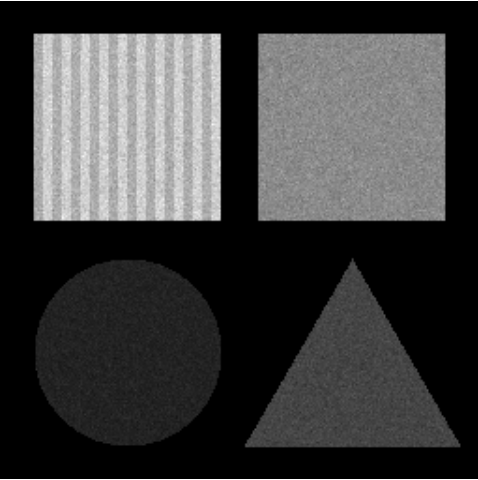
\includegraphics[width=0.65\textwidth]{../bilder/1_1.png}
\caption{Erstellte Szintigramm-Simulation für Aufgabe 1.1.}
\label{1_1}
\end{figure}

\chapter{Aufgabenblock 2}
\section{}
\begin{itemize}
\item \textbf{Aufgabe:} Grauwertprofile bei y-Werten 60 und -60 erstellen.
\item \textbf{Lösung:} Siehe Abbildungen \ref{2_1_1} und \ref{2_1_2}.
\end{itemize}

\begin{figure}[h]
\centering
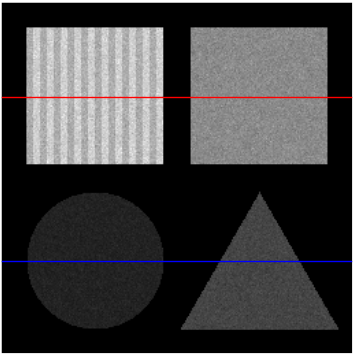
\includegraphics[width=0.65\textwidth]{../bilder/profillagen.png}
\caption{Die Lage der Grauwertprofile aus Aufgabe 2.1.}
\label{2_1_1}
\end{figure}

\begin{figure}[h]
\centering
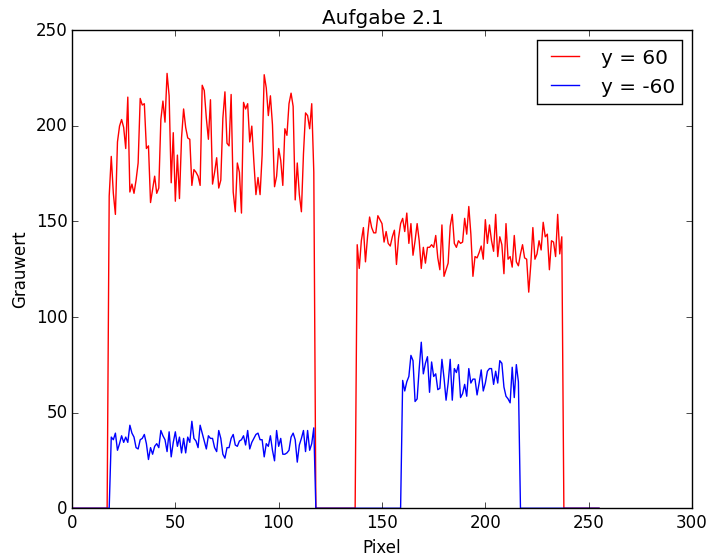
\includegraphics[width=\textwidth]{../bilder/profile.png}
\caption{Der in Aufgabe 2.1 gefragte Profilverlauf.}
\label{2_1_2}
\end{figure}

\section{}
\begin{itemize}
\item \textbf{Aufgabe:} Erstellen des Grauwert-Histogramms für das Bild aus 1.1.
\item \textbf{Lösung:} Das Histogramm ist als Abbildung \ref{2_2} zu finden.
\end{itemize}

\begin{figure}[h]
\centering
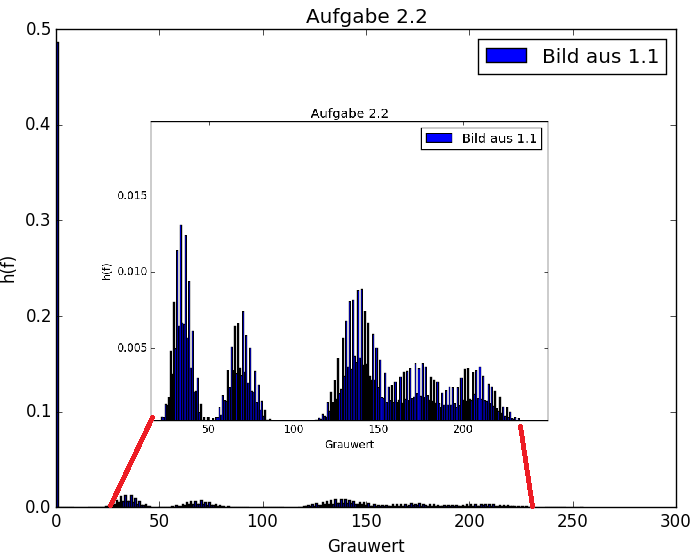
\includegraphics[width=\textwidth]{../bilder/hist.png}
\caption{Histogramm zum Bild aus Abbildung \ref{1_1}.}
\label{2_2}
\end{figure}

\section{}
\begin{itemize}
\item \textbf{Aufgabe:} Zu berechnen sind Mittelwert und Schiefe für das Grauwert-Histogramm aus Aufgabe 2.2.
\item \textbf{Lösung:} Die entsprechenden Werte sind in Tabelle \ref{mean_skew} zu finden.
\end{itemize}

\section{}
\begin{itemize}
\item \textbf{Aufgabe:} Es ist der mittlere Informationsgehalt pro Pixel des Bildes aus Aufgabe 1.1 zu ermitteln.
\item \textbf{Lösung:} Entsprechend $\bar{I} = -\sum h(f) * ld[h(f)]$ ergibt sich der mittlere Informationsgehalt zu $4,655$.
\end{itemize}

\section{}
\begin{itemize}
\item \textbf{Aufgabe:} Erstellen aller Bitebenen des Bildes aus Aufgabe 1.1, sowie die Berechnung des mittleren Informationsgehaltes aller Ebenen. Welche Bitebenen enthalten sinnvolle Information?
\item \textbf{Lösung:} Die Bitebenen sind in Abbildung \ref{bitlayer} dargestellt. Bloße Betrachung vermittelt den Eindruck, dass sich die Flächenquellen nur in den Bitebenen 5 bis 7 voneinander unterscheiden lassen, davor also keine nützliche Information zustande kommt. Dieser Eindruck wird durch das Ergebnis der Addition von Ebenen 5 bis 7 verstärkt, zu sehen in Abbildung \ref{bitlayer_3}. Mit nur diesen drei Ebenen wird bereits ein nahezu vollständiger Bildeindruck erreicht. Der jeweilige mittlere Informationsgehalt ist Tabelle \ref{bit_mean_info} zu entnehmen.
\end{itemize}

\begin{figure}[h]
\centering
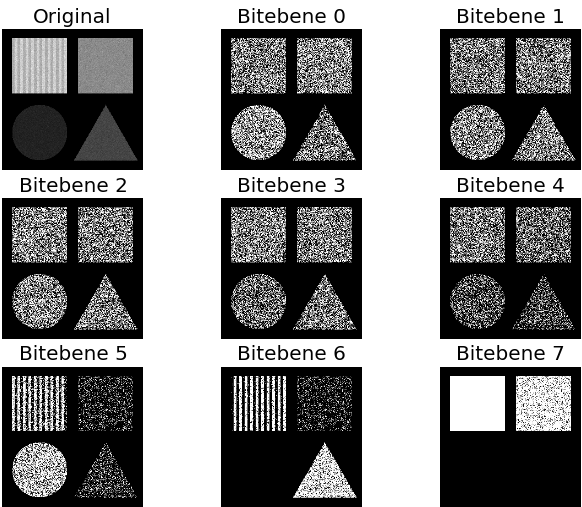
\includegraphics[width=\textwidth]{../bilder/bitebenen.png}
\caption{Bitebenen 0 bis 7 des Bildes aus Aufgabe 1.1.}
\label{bitlayer}
\end{figure}


\begin{figure}[h]
\centering
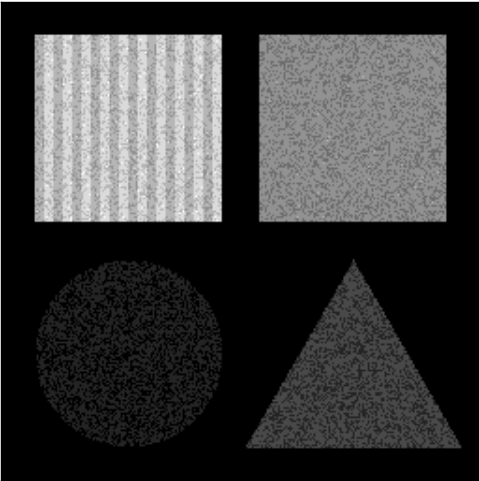
\includegraphics[width=0.65\textwidth]{../bilder/bitebenen_3.png}
\caption{Das Ergebnis der werterichtigen Addition der Bitebenen 5 bis 7.}
\label{bitlayer_3}
\end{figure}

\begin{table}
\centering
\begin{tabular}{c|c|c|c|c|c|c|c|c}
Bitebene & 0 & 1 & 2 & 3 & 4 & 5 & 6 & 7 \\ 
\hline 
$\bar{I}$ & 0,910  & 0,912 & 0,911 & 0,901 & 0,859 & 0,863 & 0,825 & 0,935 \\ 
\end{tabular}
\caption{Mittlerer Informationsgehalt für alle Bitebenen des Bildes aus Aufgabe 1.1.}
\label{bit_mean_info}
\end{table}

\section{}
\begin{itemize}
\item \textbf{Aufgabe:} Es soll ein zeilenweises Differenzbild des simulierten Szintigramms erzeugt werden. Anschließend soll auf dieser Basis ein Histogramm und der mittlere Informationsgehalt bestimmt und mit den Ergebnissen aus 2.4 verglichen werden.
\item \textbf{Lösung:} Das Differenzbild sowie das zugehörige Histogramme sind in den Abbildungen \ref{diff_img} und \ref{diff_hist} zu finden. Die Berechnung des mittleren Informationsgehalts führt auf einen Wert von 3,583. Der Unterschied bei Histogramm und mittlerem Informationsgehalt ist natürlich miteinander verbunden: Durch den stark verringerten Histogrammumfang, also eine kleinere Palette an Grauwerten, nehmen mehr Pixel den gleichen Wert an. Das führt zu sinkender mittlerer Information, wie man sich leicht anhand des Extrembeispiels eines Bildes mit nur einem Grauwert überlegen kann.
\end{itemize}

\begin{figure}[h]
\centering
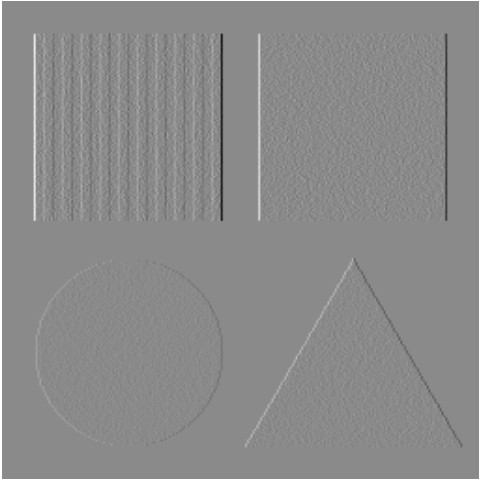
\includegraphics[width=0.65\textwidth]{../bilder/diff_img.png}
\caption{Zeilenweises Differenzbild zu Abbildung \ref{1_1}.}
\label{diff_img}
\end{figure}

\begin{figure}[h]
\centering
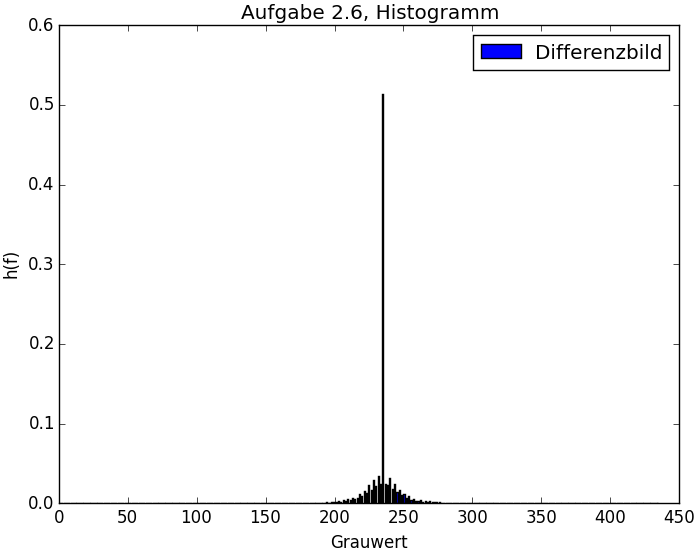
\includegraphics[width=\textwidth]{../bilder/diff_hist.png}
\caption{Histogramm zu Abbildung \ref{diff_img}, bei Berücksichtigung von Pixeln mit Wert 0.}
\label{diff_hist}
\end{figure}

\section{}
\begin{itemize}
\item \textbf{Aufgabe:} Man berechne die 2D Fouriertransformierte und das Leistungsspektrum aus Aufgabe 1.1.
\item \textbf{Lösung:} In den Abbildungen \ref{ft} und \ref{leistung} ist der Absolutbetrag der Fouriertransformierten und deren Quadrat (Leistungsspektrum) abgebildet.
\end{itemize}

\begin{figure}[h]
\centering
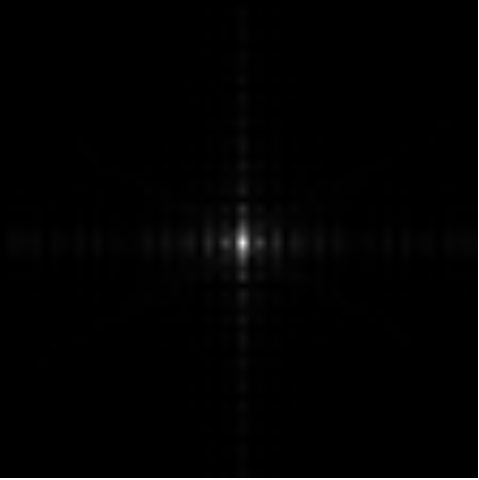
\includegraphics[width=0.65\textwidth]{../bilder/ft.png}
\caption{Absolutbetrag der Fouriertransformierten des Bildes aus 1.1.}
\label{ft}
\end{figure}

\begin{figure}[h]
\centering
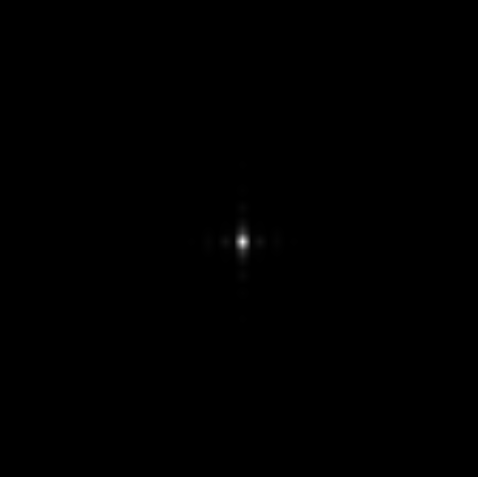
\includegraphics[width=0.65\textwidth]{../bilder/leistungsspektrum.png}
\caption{Das Leistungsspektrum des Bildes aus 1.1.}
\label{leistung}
\end{figure}

\section{}
\begin{itemize}
\item \textbf{Aufgabe:} Das Bild aus 1.1 ist um 30$^\circ$ zu drehen und anschließend die Fouriertransformierte zu berechnen.
\item \textbf{Lösung:} Siehe Abbildung \ref{ft_rot}. Da die 2D-Fouriertransformation zu Linien im Ortsraum immer senkrecht dazu stehende Linien im Frequenzraum erzeugt, muss eine Drehung im Ortsraum zu einer identischen Drehung im Frequenzraum führen. Dieses Verhalten kann auch im vorliegenden Beispiel beobachtet werden.
\end{itemize}

\begin{figure}[h]
\centering
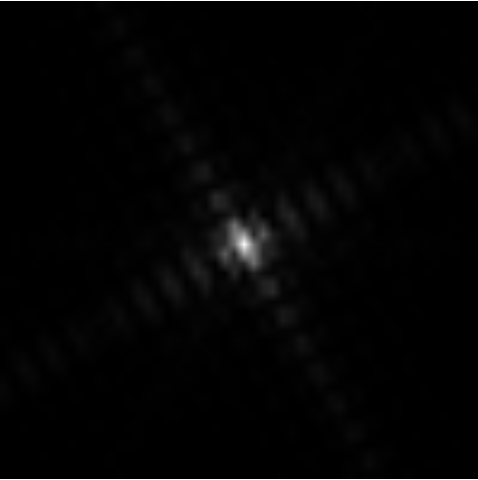
\includegraphics[width=0.65\textwidth]{../bilder/ft_rotation.png}
\caption{Der Absolutwert der Fouriertransformierten des um 30$^\circ$ gedrehten Bildes aus 1.1}
\label{ft_rot}
\end{figure}

\section{bis \hspace{2 pt} 2.11}
\begin{itemize}
\item \textbf{Aufgabe:} Es sollen ein Tief-, Band- und Hochpassfilter jeweils auf das Bild aus Aufgabe 1.1 angewendet werden.
\item \textbf{Lösung:} Die entsprechenden Ergebnisse sind in den Abbildungen \ref{tief}, \ref{band} und \ref{hoch} zu sehen und entsprechen den Erwartungen. Der Tiefpass verschmiert die Kanten der Flächenquellen im Bild, lässt aber die homogenen Flächen erkennbar. Der Bandpassfilter betont die Kanten, in Flächenquelle B sind aber noch ansatzweise die Streifen unterschiedlicher Intensität zu sehen. Der Hochpassfilter schließlich erhält quasi nur noch die Quellenkanten und das hochfrequente Rauschen innerhalb der Quellen.
\end{itemize}

\begin{figure}[h]
\centering
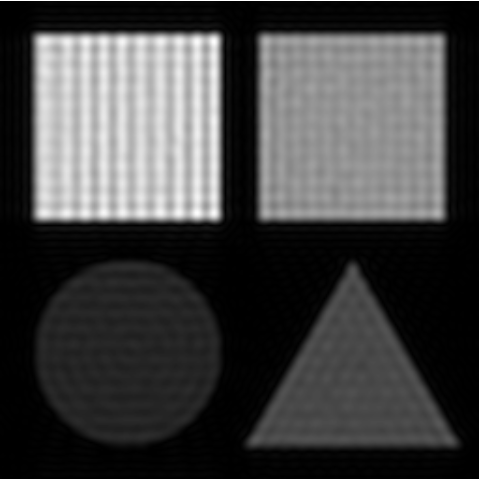
\includegraphics[width=0.65\textwidth]{../bilder/tiefpass.png}
\caption{Tiefpass, angewendet auf das Bild aus 1.1.}
\label{tief}
\end{figure}

\begin{figure}[h]
\centering
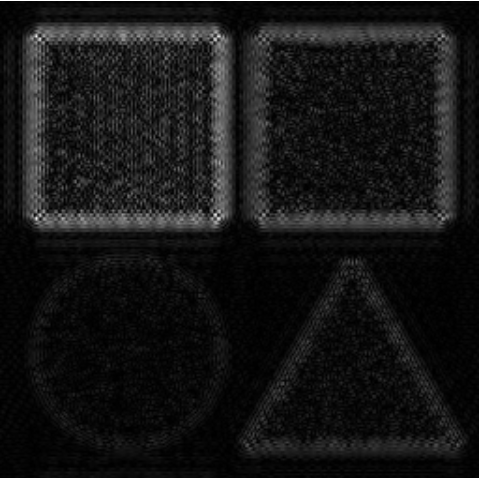
\includegraphics[width=0.65\textwidth]{../bilder/bandpass.png}
\caption{Bild aus 1.1 nach Bandpassfilterung.}
\label{band}
\end{figure}

\begin{figure}[h]
\centering
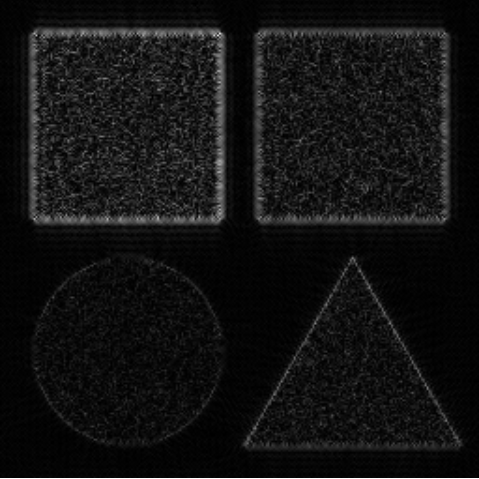
\includegraphics[width=0.65\textwidth]{../bilder/hochpass.png}
\caption{Hochpassgefiltertes Bild aus Aufgabe 1.1.}
\label{hoch}
\end{figure}

\chapter{Aufgabenblock 3}

\section{}
\begin{itemize}
\item \textbf{Aufgabe:} Es sollen verschiedene Kennlinien auf einen zu programmierenden Graukeil angewendet werden.
\item \textbf{Lösung:} Siehe Abbildung \ref{gray}. Die Wirkung der Kennlinien erschließt sich jeweils aus der mathematischen Abbildung: Die inverse Kennlinie vertauscht einfach die hohen und niedrigen Grauwerte. Die quadratische bzw. die Wurzelkennlinie strecken den dunklen bzw. hellen Bereich, die binäre Kennlinie führt zu einem binären Bild je nach Schwellwert, und die Gauß-Kennlinie streckt leicht den mittleren Bereich.
\end{itemize}

\begin{figure}
\centering
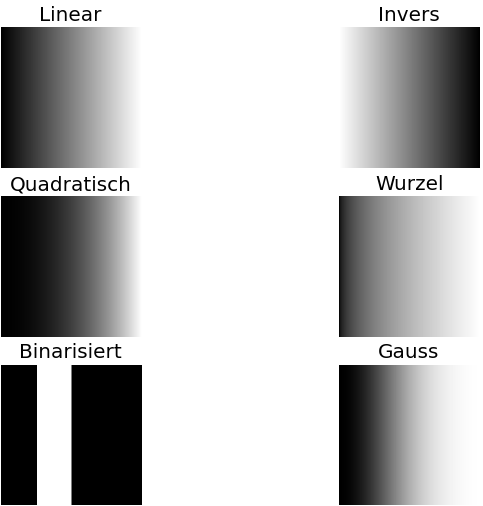
\includegraphics[width=\textwidth]{../bilder/graukeil.png}
\caption{Linearer Graukeil mit 256 Grauwerten, im Original und nach Anwendung unterschiedlicher Kennlinien}
\label{gray}
\end{figure}

\section{}
\begin{itemize}
\item \textbf{Aufgabe:} Das Bild aus 1.1 soll um 90$^\circ$ gedreht werden und dann mit der im Skript hergeleiteten Scherungsmatrix manipuliert werden.
\item \textbf{Lösung:} Zu sehen in Abbildung \ref{scherung}
\end{itemize}

\begin{figure}
\centering
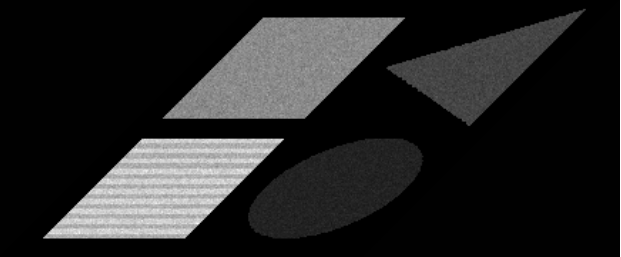
\includegraphics[width=\textwidth]{../bilder/scherung.png}
\caption{Das gedrehte und gescherte Bild.}
\label{scherung}
\end{figure}

\section{}
\begin{itemize}
\csname c@topnumber\endcsname=0
\item \textbf{Aufgabe:} Das Bild 1.1 soll mit verschiedenen Filtern (Mittelwert, Median, Binomial) bearbeitet werden. Alle Filter sollen einen Filterkern von 3x3 Pixeln verwenden. Eventuelle Unterschiede sollen anhand von Profilen diskutiert werden.
\item \textbf{Lösung:} Für die Bilder siehe Abbildungen \ref{mmb} und \ref{mmb_profil}. Gerade am Profilverlauf über der Flächenquelle B mit Streifen unterschiedlicher Aktivität zeigen sich Unterschiede. Prinzipbedingt kann eine Mittelwertsfilterung diese Kanten nur eingeschränkt erhalten. Schon besser gelingt dies mit dem Binomialfilter (gewichteter Mittelwert), nur das Medianfilter erhält die Kanten jedoch auch nach mehrmaliger Filterung.
\end{itemize}

\begin{figure}
\centering
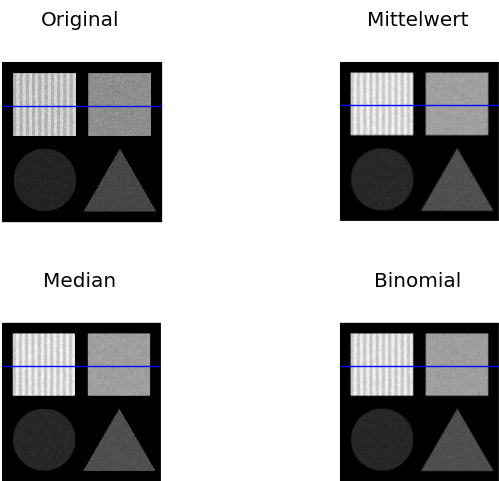
\includegraphics[width=\textwidth]{../bilder/mmb_lage.png}
\caption{Die Ergebnisse unterschiedlicher Filter und die Lage des als nächstes betrachteten Profils.}
\label{mmb}
\end{figure}

\begin{figure}
\centering
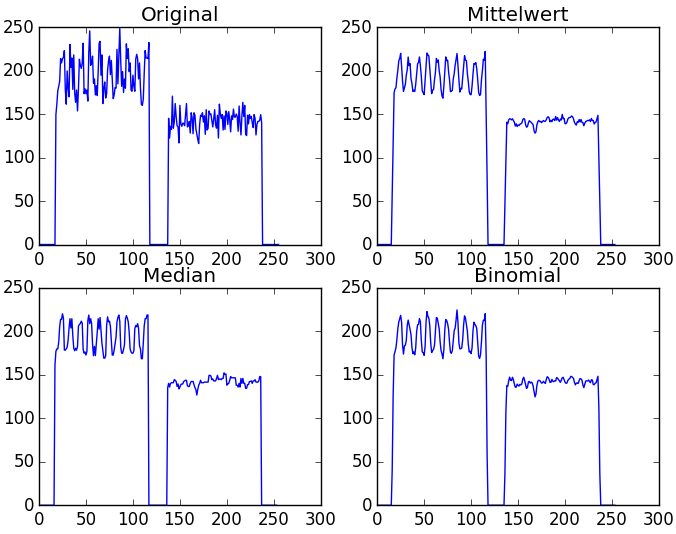
\includegraphics[width=\textwidth]{../bilder/mmb_profile.png}
\caption{Die Grauwert-Verläufe nach unterschiedlichen Filtern.}
\label{mmb_profil}
\end{figure}

\section{}
\begin{itemize}
\item \textbf{Aufgabe:} Es sollen das Sobel- und Roberts-Filter angewendet werden, eventuell auftretende Unterschiede sind zu erklären.
\item \textbf{Lösung:} Die Ergebnisbilder sind in der Abbildung \ref{sobel} zu sehen. Es fällt auf dass das Roberts-Filter zu einer blasseren, schärferen Abbildung führt, wohl aufgrund der geringen Filterkerngröße und der fehlenden Wichtung.
\end{itemize}

\begin{figure}[h]
\centering
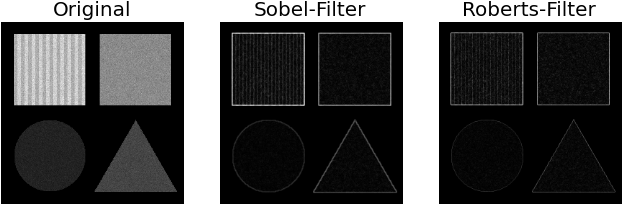
\includegraphics[width=\textwidth]{../bilder/sobel_roberts.png}
\caption{Das Ergebnis der Sobel- und Roberts-Filter.}
\label{sobel}
\end{figure}

\section{}
\begin{itemize}
\item \textbf{Aufgabe:} Ein Laplace-Filter (8er Nachbarschaft) ist auf das Bild 1.1 anzuwenden. Eventuelle Unterschiede sollen im Vergleich zu 3.4 diskutiert werden.
\item \textbf{Lösung:} Abbildung \ref{laplace} zeigt das Ergebnis der Filterung. Bei genauerer Betrachtung wird deutlich, dass die Flächenquellen nach dem Laplacefilter deutlich inhomogener erscheinen als bei Sobel- oder Roberts-Filter. Dieses Verhalten ist in der Tat zu erwarten, da die zweite Ableitung deutlich anfälliger für das statistische Rauschen innerhalb der Flächenquellen ist.
\end{itemize}

\begin{figure}[h]
\centering
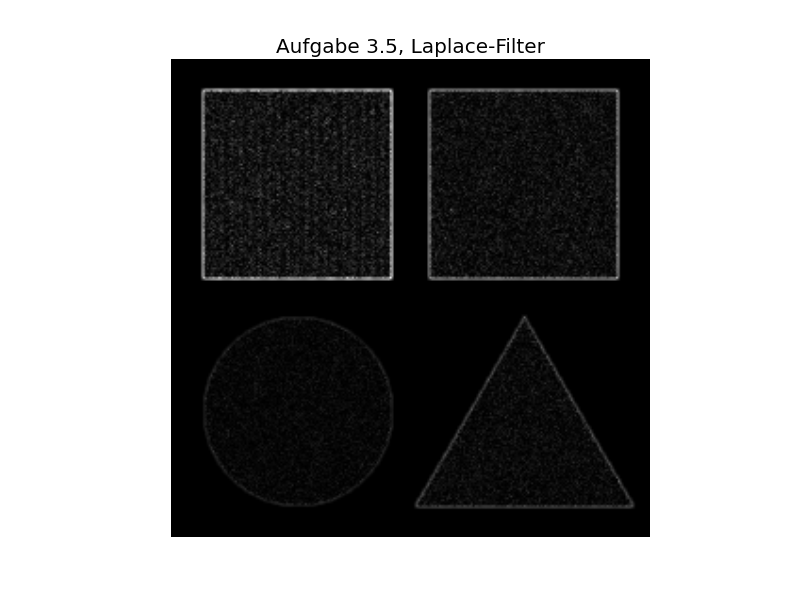
\includegraphics[width=\textwidth]{../bilder/laplace_abs.png}
\caption{Ergebnis des 8er Laplace Filters. Dargestellt sind die absoluten Grauwerte, um bessere Vergleichbarkeit mit Aufgabe 3.4 zu gewährleisten}
\label{laplace}
\end{figure}

\section{}
\begin{itemize}
\item \textbf{Aufgabe:} Die Flächenquelle D im Bild 1.1 soll per Schwellwert vom Rest des Bildes isoliert werden.
\item \textbf{Lösung:} Siehe Abbildung \ref{schwellwert}.
\end{itemize}

\begin{figure}[h]
\centering
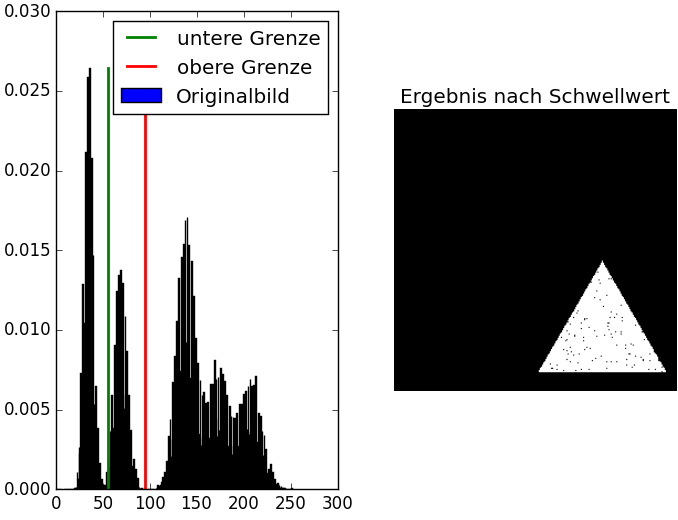
\includegraphics[width=\textwidth]{../bilder/schwellwert.png}
\caption{Ergebnis einer Binarisierung mit Schwellwerten 55 und 95, basierend auf der Verteilung im Histogramm.}
\label{schwellwert}
\end{figure}

\section{}
\begin{itemize}
\csname c@topnumber\endcsname=0
\item \textbf{Aufgabe:} Es soll die Hough-Transformation des rechten unteren Quadranten durchgeführt werden.
\item \textbf{Lösung:} Nach hierzu geeigneter Filterung zur Kantenextraktion wird der Algorithmus zur Hough-Transformation angewendet. Die Ergebnisse sind in den Abbildungen \ref{hough_img} und \ref{hough_graph} zu sehen. Die 2D-Darstellung bietet den aus der Vorlesung bekannten Überblick, wärend der Graph das Erkennen der Häufungspunkte besonders leicht macht. Wie für ein gleichseitiges Dreieck zu erwarten, finden sich Häufungspunkte bei 30$^\circ$, 90$^\circ$ und 150$^\circ$.
\end{itemize}

\begin{figure}[h]
\centering
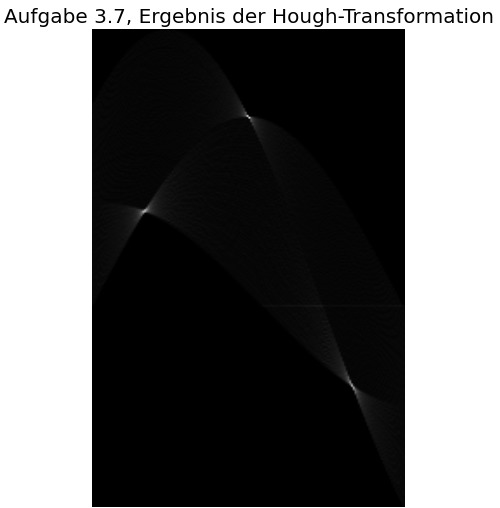
\includegraphics[width=0.65\textwidth]{../bilder/hough_1.png}
\caption{Ausgabe der Hough-Transformation. Die Häufungspunkte entsprechen den Winkeln, bei denen Kanten erkannt wurden.}
\label{hough_img}
\end{figure}

\begin{figure}[h]
\centering
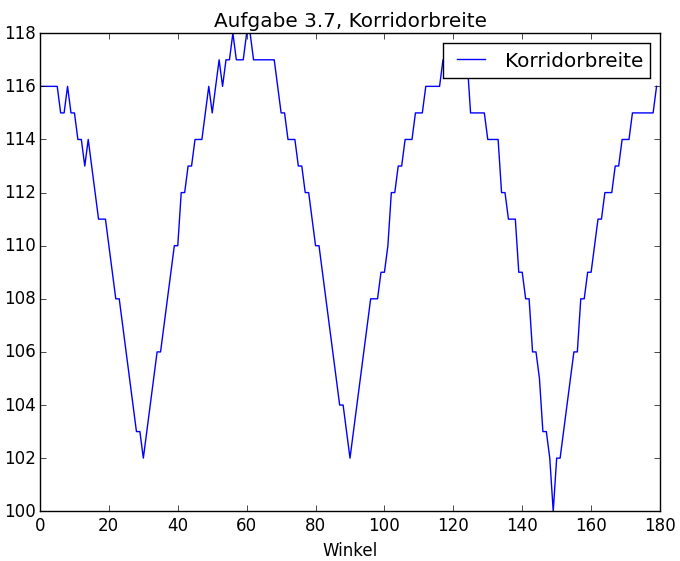
\includegraphics[width=\textwidth]{../bilder/hough_2.png}
\caption{Plot der selbst eingeführten "Korridorbreite", die Anzahl der Pixel im vorherigen Hough-Diagramm mit $f > 0$ pro Winkel. Hierin sind die Häufungswinkel besonders leicht abzulesen.}
\label{hough_graph}
\end{figure}

\section{}
\begin{itemize}
\item \textbf{Aufgabe:} Es sind der geometrische und der Massenschwerpunkt des Objekts bestehend aus den Flächenquellen B und C zu berechnen.
\item \textbf{Lösung:} Die Lage der beiden Schwerpunkte ist in Abbildung \ref{schwerpunkt} dargestellt. Der geometrische Schwerpunkt liegt erwartungsgemäß nur leicht exzentrisch, der Massenschwerpunkt hingegen voll auf Quelle B. Aufgrund der stark unterschiedlichen Grauwerte ist die Quelle B erheblich "schwerer". In Pixelkoordinaten des Teilbildes liegt der geometrische Schwerpunkt bei (63,120) und der Massenschwerpunkt bei (63,83), bei Koordinatenursprung in der linken oberen Bildecke (numpy-Array-Indexierung).
\end{itemize}

\begin{figure}[h]
\centering
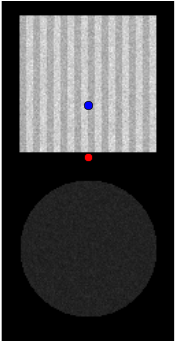
\includegraphics[width=0.5\textwidth]{../bilder/schwerpunkte.png}
\caption{Zu sehen ist in rot der geometrische Schwerpunkt und in blau der Massenschwerpunkt des Bildes.}
\label{schwerpunkt}
\end{figure}

\section{}
\begin{itemize}
\csname c@topnumber\endcsname=0
\item \textbf{Aufgabe:} Die Textur der Flächenquelle B soll nach Filterung mit einem geeigneten Filter anhand einer Grauwert-Übergangsmatrix berechnet werden. Hierzu sind zwei Verschiebungsvektoren, (1,0) und (0,1), zu verwenden.
\item \textbf{Lösung:} Das verwendete Ausgangsbild sowie die Übergangsmatrizen zu beiden Verschiebungsvektoren sind in Abbildung \ref{transition} zu finden. Die in beiden Fällen stark besetzte Hauptdiagonale bestätigt den unmittelbaren Bildeindruck: Es sind hauptsächlich große, homogene Flächen vorhanden. Die unterbrochene Linie in der Hauptdiagonalen der Matrix zum Vektor (1,0) kommt dadurch zustande, dass hier auch die Quadranten rechts oben und links unten leicht besetzt sind, wobei die Intensität aber die Hauptdiagonale nicht erreicht und darum weitgehend unsichtbar bleibt.
\end{itemize}

\begin{figure}[h]
\centering
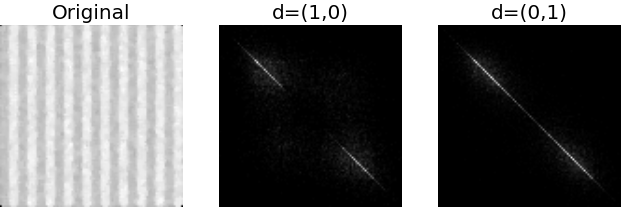
\includegraphics[width=\textwidth]{../bilder/transition_matrix.png}
\caption{Übergangsmatrix zu den Verschiebungsvektoren (1,0) (Mitte) und (0,1) (rechts).}
\label{transition}
\end{figure}


\end{document}